\begin{figure}[h]
  \subfloat[\mad internal net example]{
    \fcolorbox{black!20}{white}{
      \begin{minipage}[c][4cm][c]{0.33\linewidth}%
        \centering
        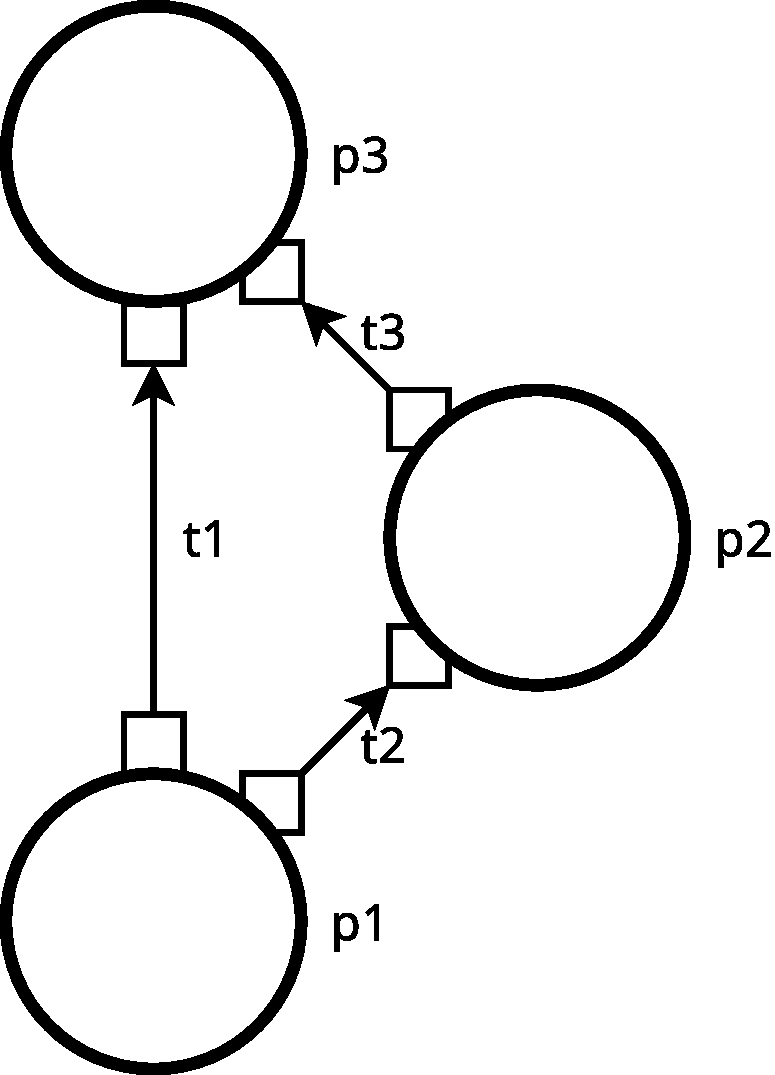
\includegraphics[width=0.8\columnwidth]{images/perf_transition.pdf} \label{fig:transmadeus}
      \end{minipage}
    }
  }
  \subfloat[Dependency graph]{
    \fcolorbox{black!20}{white}{
      \begin{minipage}[c][4cm][c]{0.53\linewidth}%
        \centering
        \begin{tikzpicture}[node distance=1.7cm]
          \node (p3) [] {$v_\text{p3}^\text{reach}$};
          \node (t1) [below =15pt of p3] {$v_\text{t1}^\text{fire}$};
          \node (p1) [below =15pt of t1] {$v_\text{p1}^\text{reach}$};
          \node (t2) [right =25pt of p1] {$v_\text{t2}^\text{fire}$};
          \node (p2) [above =15pt of t2] {$v_\text{p2}^\text{reach}$};
          \node (t3) [above =15pt of p2] {$v_\text{t3}^\text{fire}$};
          \draw [->] (t3) -- (p3) node[midway, above, scale=0.7] {$t(\text{t3})$};
          \draw [->] (t2) -- (p2) node[midway, right, scale=0.7] {$t(\text{t2})$};
          \draw [->] (t1) -- (p3) node[midway, right, scale=0.7] {$t(\text{t1})$};
          \draw [->] (p1) -- (t1) node[midway, right, scale=0.7] {$0$};
          \draw [->] (p1) -- (t2) node[midway, above, scale=0.7] {$0$};
          \draw [->] (p2) -- (t3) node[midway, right, scale=0.7] {$0$};
        \end{tikzpicture}
        \label{fig:transdag}
      \end{minipage}
    }
  }
  \caption{A set of \mad transitions and their corresponding equivalent dependency graph}
  \label{fig:transition_graph}
\end{figure}
